\PassOptionsToPackage{unicode=true}{hyperref} % options for packages loaded elsewhere
\PassOptionsToPackage{hyphens}{url}
%
\documentclass[]{book}
\usepackage{lmodern}
\usepackage{amssymb,amsmath}
\usepackage{ifxetex,ifluatex}
\usepackage{fixltx2e} % provides \textsubscript
\ifnum 0\ifxetex 1\fi\ifluatex 1\fi=0 % if pdftex
  \usepackage[T1]{fontenc}
  \usepackage[utf8]{inputenc}
  \usepackage{textcomp} % provides euro and other symbols
\else % if luatex or xelatex
  \usepackage{unicode-math}
  \defaultfontfeatures{Ligatures=TeX,Scale=MatchLowercase}
\fi
% use upquote if available, for straight quotes in verbatim environments
\IfFileExists{upquote.sty}{\usepackage{upquote}}{}
% use microtype if available
\IfFileExists{microtype.sty}{%
\usepackage[]{microtype}
\UseMicrotypeSet[protrusion]{basicmath} % disable protrusion for tt fonts
}{}
\IfFileExists{parskip.sty}{%
\usepackage{parskip}
}{% else
\setlength{\parindent}{0pt}
\setlength{\parskip}{6pt plus 2pt minus 1pt}
}
\usepackage{hyperref}
\hypersetup{
            pdftitle={Takrar},
            pdfauthor={Sumeed Manzoor},
            pdfborder={0 0 0},
            breaklinks=true}
\urlstyle{same}  % don't use monospace font for urls
\usepackage{longtable,booktabs}
% Fix footnotes in tables (requires footnote package)
\IfFileExists{footnote.sty}{\usepackage{footnote}\makesavenoteenv{longtable}}{}
\usepackage{graphicx,grffile}
\makeatletter
\def\maxwidth{\ifdim\Gin@nat@width>\linewidth\linewidth\else\Gin@nat@width\fi}
\def\maxheight{\ifdim\Gin@nat@height>\textheight\textheight\else\Gin@nat@height\fi}
\makeatother
% Scale images if necessary, so that they will not overflow the page
% margins by default, and it is still possible to overwrite the defaults
% using explicit options in \includegraphics[width, height, ...]{}
\setkeys{Gin}{width=\maxwidth,height=\maxheight,keepaspectratio}
\setlength{\emergencystretch}{3em}  % prevent overfull lines
\providecommand{\tightlist}{%
  \setlength{\itemsep}{0pt}\setlength{\parskip}{0pt}}
\setcounter{secnumdepth}{5}
% Redefines (sub)paragraphs to behave more like sections
\ifx\paragraph\undefined\else
\let\oldparagraph\paragraph
\renewcommand{\paragraph}[1]{\oldparagraph{#1}\mbox{}}
\fi
\ifx\subparagraph\undefined\else
\let\oldsubparagraph\subparagraph
\renewcommand{\subparagraph}[1]{\oldsubparagraph{#1}\mbox{}}
\fi

% set default figure placement to htbp
\makeatletter
\def\fps@figure{htbp}
\makeatother

\usepackage{booktabs}
\usepackage{amsthm}
\usepackage{cancel}
% \usepackage{fontspec}
% \usepackage{polyglossia}
% \setmainlanguage{english}
% \setotherlanguage{arabic}
\newfontfamily\arabicfont[Script = Arabic]{Amiri Quran} % Replace 'Simplified Arabic' with a font from your system
\usepackage{arabtex}
\usepackage{utf8}
\usepackage{multirow}
\makeatletter
\def\thm@space@setup{%
  \thm@preskip=8pt plus 2pt minus 4pt
  \thm@postskip=\thm@preskip
}
\makeatother
\setcode{utf8}
\usepackage{cancel}
\usepackage{booktabs}
\usepackage{longtable}
\usepackage{array}
\usepackage{multirow}
\usepackage{wrapfig}
\usepackage{float}
\usepackage{colortbl}
\usepackage{pdflscape}
\usepackage{tabu}
\usepackage{threeparttable}
\usepackage{threeparttablex}
\usepackage[normalem]{ulem}
\usepackage{makecell}
\usepackage{xcolor}
\usepackage[]{natbib}
\bibliographystyle{apalike}

\title{Takrar}
\author{Sumeed Manzoor}
\date{last compiled on 2021-09-10 00:02:47}

\begin{document}
\maketitle

{
\setcounter{tocdepth}{1}
\tableofcontents
}
\hypertarget{intro}{%
\chapter{Introduction}\label{intro}}

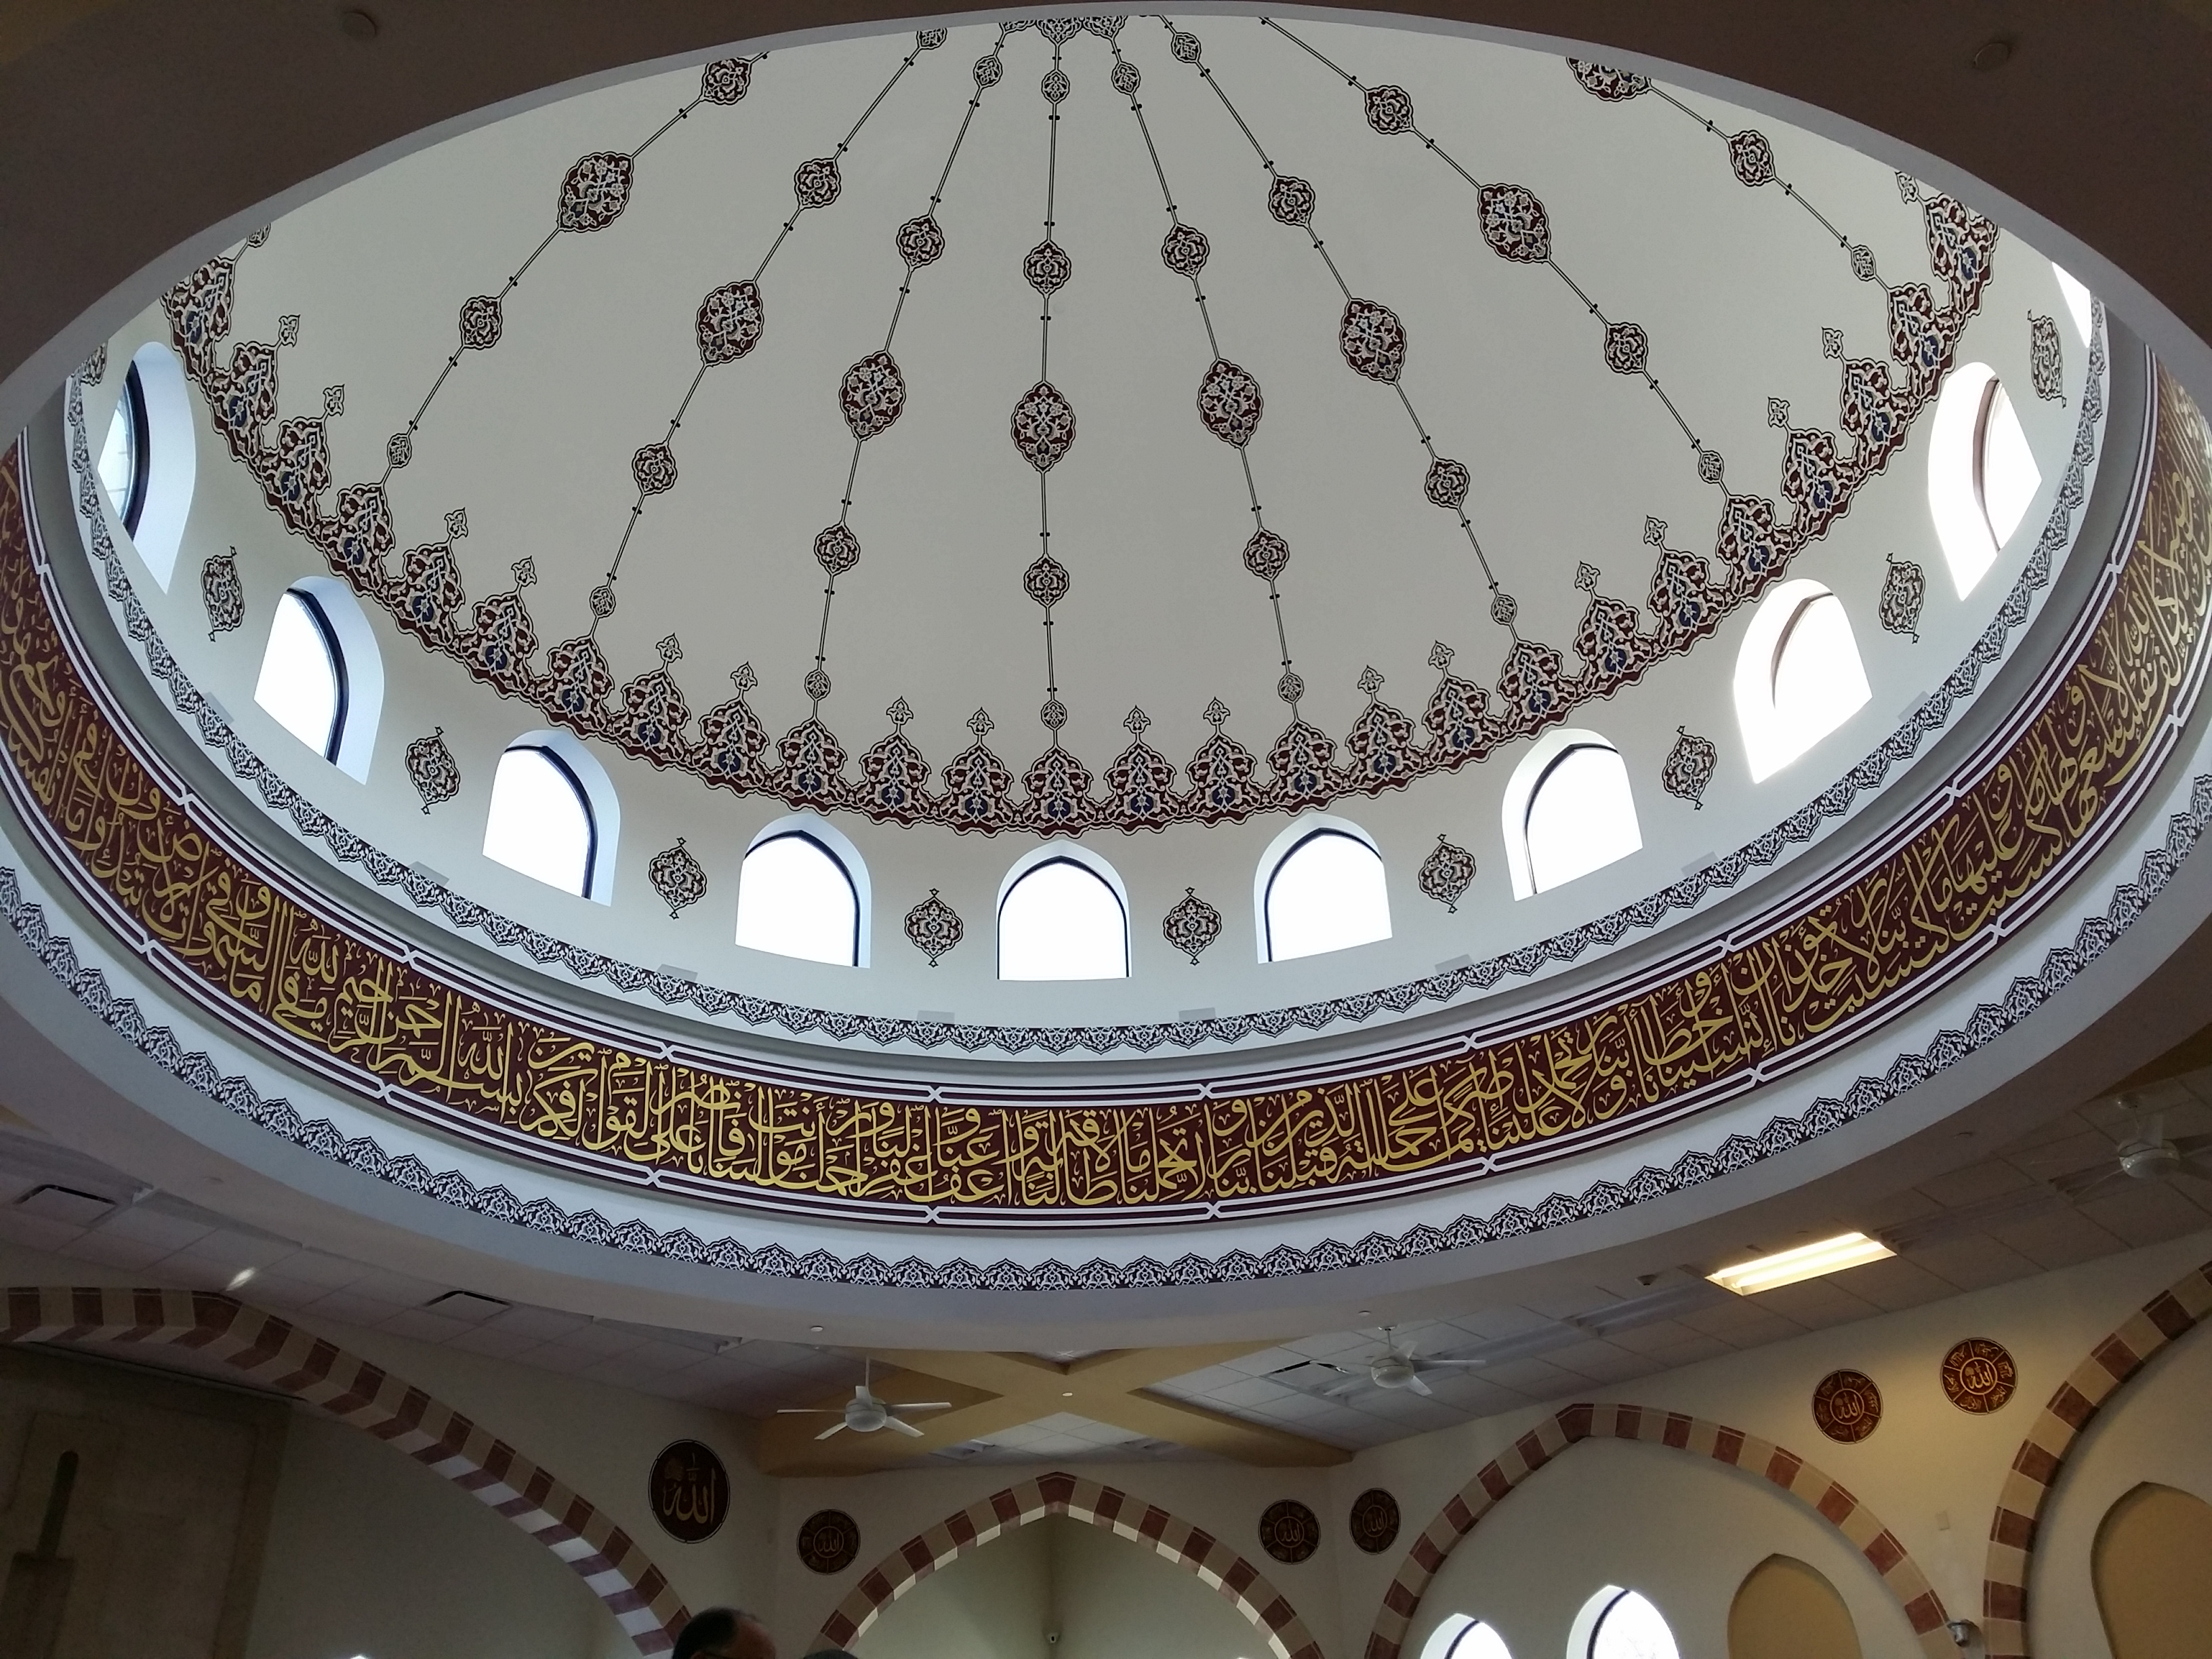
\includegraphics{images/ds2.jpg}

\hypertarget{intent}{%
\section{Intentions}\label{intent}}

This is a lengthy topic, and not one I can do justice to with my limited amount of knowledge and in the time I have to write this. Indeed, renewing intentions is a continuous and iterative exercise, and perhaps this sections should be similarly continuously revised. For now, I will repeat what Mufti Azeem shared on the 8/17/21 Tuesday night tafseer.\\
While seeking and attaining knowledge, we should have several key intentions:

\begin{itemize}
\tightlist
\item
  To remove all bad desires
\item
  We make du'a that the topic we're learning will provide solace to difficulties we are dealing with in our life
\item
  We act on what we learn and teach it to others
\end{itemize}

\hypertarget{seeking-knowledge}{%
\section{Seeking knowledge}\label{seeking-knowledge}}

\begin{quote}
\textbf{العلم بلا عملٍ}\\
\textbf{كالشجرة بلا ثمرٍ}
\end{quote}

\begin{quote}
Knowledge without action\\
Is like the tree that doesn't bear fruit
\end{quote}

علم is composed of two things: knowledge \emph{and} action.

To attain علم, tarbiyya is extremely important. Imam Shafi'i narrates this poem about the advice of his teacher, Waki'i:

\begin{quote}
شَكَوْتُ إلَى وَكِيعٍ سُوءَ حِفْظِي\\
فَأرْشَدَنِي إلَى تَرْكِ المعَاصي\\
وَأخْبَرَنِي بأَنَّ العِلْمَ نُورٌ
ونورُ الله لايؤتى لعاصي
\end{quote}

\begin{quote}
I complained to Waki' about my memory
He advised me to leave my sins
He advised me that it is because knowledge is a light
And the the light of Allah ﷻ does not come to a sinner
\end{quote}

Imam Malik says:

\begin{quote}
العلم و الحكمة نور\\
يهد الله به من يشاء\\
و ليس كثرة المسائل
\end{quote}

\begin{quote}
Knowledge and wisdom are light\\
that Allah ﷻ uses to guide who he wills\\
and they are not answering a lot of questions
\end{quote}

The purpose of seeking knowledge is not to be able to answer difficult questions people ask of us, or to argue against others. It is a light that we pray guides us to find nearness to Allah ﷻ.

\hypertarget{conversation}{%
\chapter{حوار}\label{conversation}}

\hypertarget{ux627ux644ux623ux633ux645ux627ux621-ux627ux644ux623ux639ux645ux627ux644}{%
\section{الأسماء الأعمال}\label{ux627ux644ux623ux633ux645ux627ux621-ux627ux644ux623ux639ux645ux627ux644}}

\begin{table}[]
\begin{tabular}{lr}
\multicolumn{1}{c}{\textbf{معنى}} & \multicolumn{1}{c}{\textbf{كلمة}} \\
\multicolumn{2}{c}{\textbf{islam/religion}}                           \\
speaker of the Masjid             & خطيب المسجد                       \\
Imam                              & امام                              \\
Muhaddith                         & محدّث                             \\
\multicolumn{2}{c}{\textbf{healthcare}}                               \\
doctor                            & طَبِيبٌ                           \\
surgeon                           & حرّاح                             \\
nurse                             & مُمَرِّضٌ                         \\
dentist                           & دكتور الاسنان                     \\
pharmacist                        & صَيْدَلِي                         \\
\multicolumn{2}{c}{\textbf{government/law}}                           \\
judge                             & قاضي                              \\
lawyer                            & مُحَامِيٌ                         \\
police officer                    & شُرْطِيٌّ                         \\
king                              & مالك                              \\
\multicolumn{2}{c}{\textbf{humanities}}                               \\
writer                            & كاتب                              \\ \hline
\multicolumn{1}{|l|}{poet}        & \multicolumn{1}{r|}{شاعر}         \\ \hline
\multicolumn{1}{|l|}{actor}       & \multicolumn{1}{r|}{ممثل}         \\ \hline
\multicolumn{1}{|l|}{journalist}  & \multicolumn{1}{r|}{صحافي}        \\ \hline
artist                            & فنان                              \\
painter                           & رسّام                             \\
dancer                            & راقِص                             \\
\multicolumn{2}{c}{\textbf{engineering/aerospace}}                    \\
engineer                          & مهندس                             \\
pilot                             & طيار                              \\
electrician                       & كهربائي                           \\
plumber                           & سبَّاك                            \\
\multicolumn{2}{c}{\textbf{school/education}}                         \\
principal/manager                 & مُدِيرٌ                           \\
teacher                           & مدرّس                             \\
student                           & طالب                              \\
chemist                           & كيميائي                           \\
\multicolumn{2}{c}{\textbf{business}}                                 \\
trader                            & تاجر                              \\
salesman                          & بائع                              \\
server (at a restaurant)          & خادم المطعم                       \\
\multicolumn{2}{c}{\textbf{farming/agriculture}}                      \\
farmer                            & مُزَارِعٌ                         \\
\multicolumn{2}{c}{\textbf{skilled professions}}                      \\
bread maker/baker                 & جَبَّازٌ                          \\
shoemaker                         & إسكافي                            \\
perfumer                          & عطار                              \\
barber                            & حلّاق                             \\
\multicolumn{2}{c}{\textbf{athlete}}                                  \\
scuba diver                       & غطاس                              \\
\multicolumn{2}{c}{\textbf{wartime}}                                  \\
soldier                           & جُنْري                            \\
spy                               & مخبر                              \\
\multicolumn{2}{c}{\textbf{miscellaneous}}                            \\
secretary                         & سِكْرِتِيرِيٌ                     \\
unemployed                        & عاطل                              \\
\multicolumn{2}{c}{\textbf{haram}}                                    \\
magician                          & ساحر                             
\end{tabular}
\end{table}

معنى

كلمة

{islam/religion}

speaker of the Masjid

خطيب المسجد

Imam

امام

Muhaddith

محدّث

{healthcare}

doctor

طَبِيبٌ

surgeon

حرّاح

nurse

مُمَرِّضٌ

dentist

دكتور الاسنان

pharmacist

صَيْدَلِي

{government/law}

judge

قاضي

lawyer

مُحَامِيٌ

police officer

شُرْطِيٌّ

king

مالك

{humanities}

writer

كاتب

poet

شاعر

actor

ممثل

journalist

صحافي

artist

فنان

painter

رسّام

dancer

راقِص

{engineering/aerospace}

engineer

مهندس

pilot

طيار

electrician

كهربائي

plumber

سبَّاك

{school/education}

principal/manager

مُدِيرٌ

teacher

مدرّس

student

طالب

chemist

كيميائي

{business}

trader

تاجر

salesman

بائع

server (at a restaurant)

خادم المطعم

{farming/agriculture}

farmer

مُزَارِعٌ

{skilled professions}

bread maker/baker

جَبَّازٌ

shoemaker

إسكافي

perfumer

عطار

barber

حلّاق

{athlete}

scuba diver

غطاس

{wartime}

soldier

جُنْري

spy

مخبر

{miscellaneous}

secretary

سِكْرِتِيرِيٌ

unemployed

عاطل

{haram}

magician

ساحر

\hypertarget{part-ux62fux631ux648ux633-ux627ux644ux625ux633ux644ux627ux645}{%
\part{دروس الإسلام}\label{part-ux62fux631ux648ux633-ux627ux644ux625ux633ux644ux627ux645}}

\hypertarget{tarbiyya}{%
\chapter{تربيّة}\label{tarbiyya}}

\hypertarget{qari-siddique}{%
\section{Qari Mohammad Sayed Siddique Ahmad Bandwi}\label{qari-siddique}}

Qari Siddique Bandwi was born in Baanda, India in 1919 \citep{bundelkhand}. He was of such character and piety that when sheikh Abdul Fattah, a renowned Syrian scholar, asked Maulana Shabiq (the principal of Darul Uloom Zakariyya) about awliyah he could visit, Maulana Shabiq referred Qari Siddique Bandwi. Sheikh Abdul Fattah traveled all they way to the small city of Baanda to visit him.

Another incident regarding Qari Bandwi is when he was collecting donations for a madrasa in baanda. He was taking the train home late at night in the remote village, bringing with him the bag of funds he collected, when a group of thieves stopped him and staged a stick up. They told him to leave the money, but Qari Bandwi said he can't give the money since it did not belong to him. The thieves did not care and wanted the money anyway, so Qari Bandwi threw them the bag and said, ``let's see how far you go.'' The next day, someone came to Qari Bandwi and said there are people in the city looking for him. It was the robbers; they were unable to make their escape ― it was like there was an invisible barrier preventing them from leaving the city.

\hypertarget{the-concept-of-ux641ux64aux636}{%
\section{The concept of فيض}\label{the-concept-of-ux641ux64aux636}}

\begin{quote}
\textbf{فيض}
\emph{Hans Wehr} flood, inundation, deluge; emanation; superabundance, plenty, copiousness, abundance; stream
\emph{معنى إصطلاح} The internal Nur, from a heart
\end{quote}

Abu Bakr, one of the awliyah in Chicago, had said (paraphrased), ``There are two steps for a Mu'min to take. The first step is to squash the nafs, the second is to enter paradise. I have taken the first step, and I am waiting for the second.''

He had also said ``The one who cannot benefit from the silence of the Ulamah will not benefit from their speech.''

This is the concept of فيض. It is the moment when Angel Jibreel hugged Nabi ﷺ tightly in the cave of Hira. It is the feeling of spiritual rejuvenation felt in the presence of the awliyah. It is part and parcel to why the Islamic tradition emphasizes attainment of knowledge from scholar to student in an intimate manner, where knowledge is not just information but an exercise in connecting heart-to-heart. We hope and pray that in this manner, by staying close with those who are close to Allah ﷻ, we too can get closer to Allah ﷻ.\\
One of the scholars would invite the students to his house from Asr to Maghrib, and offer them tea. They would not say anything in that time, just sit and do Adhkar. Just by sitting in the presence of the scholar, the students could find benefit in their own spiritual growth.

\hypertarget{miracles}{%
\section{Miracles}\label{miracles}}

In the story of the theives and \protect\hypertarget{qari-siddique}{}{Qari Siddique Bandwi}, the supernatural incident where the thieves were unable to leave the city due to an invisible barrier they felt is an example of a \emph{كرامة}.\\
\textbf{معجرة} is the supernatural phenomenon for a prophet. إعجاز is literally something inimitable and wondrous. For example, Rasulullah ﷺ splitting the moon, or Musa (AS) splitting the sea.\\
\textbf{كرامة} is where a supernatural incident happens at the hands of a wali of Allah ﷻ. It honors the wali and proves their nearness to Allah ﷻ. Every كرامة is a معجرة of their prophet because they would not happen without the wali following the sunnah of their prophet.

\textbf{إرحاص} a supernatural phenomenon done by a kuffar to deceive others.\\
\textbf{إستدراج} a supernatural phenomenon that deceives oneself. It is literally to get reeled in. For example, fir'aun seeing the sea split believed that it was his ability that led to the sea being split, but it was not his ability, it was Musa (AS). By fooling himself, fir'aun found greater conviction in his ضلال.

إستدراج is extremely important for us to be aware of. درج means levels, and إستدراج works in levels, step by step people fall of the deen. For example, if someone is doing da'wah on youtube, and they start to gain a significant following, to be wary of إستدراج means to realize that the popularity could be a test of one's ego.\\
We see this wariness among the Sahaba. During the khilafa of Umar (RA), he saw the Masjid filled with gems, and gold, and riches. The Muslims were joyful, but Umar (RA) was sad. He asked if this was a blessing, why was it not given to Rasulullah ﷺ or Abu Bakr (RA)? He realized that the blessing given to him and the Muslims was a test.\\
Another example is Sulaiman (AS). The ayah in the Qur'an discusses this (27:40):

\begin{quote}
قَالَ ٱلَّذِى عِندَهُۥ عِلْمٌ مِّنَ ٱلْكِتَـٰبِ أَنَا۠ ءَاتِيكَ بِهِۦ قَبْلَ أَن يَرْتَدَّ إِلَيْكَ طَرْفُكَ ۚ فَلَمَّا رَءَاهُ مُسْتَقِرًّا عِندَهُۥ قَالَ هَـٰذَا مِن فَضْلِ رَبِّى لِيَبْلُوَنِىٓ ءَأَشْكُرُ أَمْ أَكْفُرُ ۖ وَمَن شَكَرَ فَإِنَّمَا يَشْكُرُ لِنَفْسِهِۦ ۖ وَمَن كَفَرَ فَإِنَّ رَبِّى غَنِىٌّ كَرِيمٌ
\end{quote}

\begin{quote}
Said one who had knowledge of the Book: ``I will bring it to thee within the twinkling of an eye!'' Then when (Solomon) saw it placed firmly before him, he said: ``This is by the Grace of my Lord!- to test me whether I am grateful or ungrateful! and if any is grateful, truly his gratitude is (a gain) for his own soul; but if any is ungrateful, truly my Lord is Free of all Needs, Supreme in Honour!''
\end{quote}

In summary, whenever there is a fadhal from Allah ﷻ, we should be grateful and aware that these things are a test.

\hypertarget{difficulties-in-memorizing}{%
\section{Difficulties in memorizing}\label{difficulties-in-memorizing}}

Imam Zaid Shakir said that when joined Madrasa, he was about 29. He spent an entire day memorizing the first line of his Nahw lesson. At the end of the day, he found that he forgot that single line he spent the entire day memorizing. He spent days and days on that single line.\\
It takes time to learn and memorize, and there will be times where it seems difficult or even impossible. But it is important to remember that Allah ﷻ chose us to be here, and it is by his will that we remember anything and his will that we forget, and we just need to put our most sincere and best effort forward in hopes that He will accept our efforts.

\hypertarget{intentions}{%
\section{Intentions}\label{intentions}}

See \protect\hyperlink{intent}{the section in the home page} for a more general discussion on intention.

It is of utmost importance to be sincere in our intentions. Through a noble intention, a small action becomes heavy in the scales, and through a bad intention a huge action becomes light in the scales.

tamlul mizan - scales are by weight, not number

\hypertarget{aqeedah}{%
\chapter{عقيدة}\label{aqeedah}}

\hypertarget{introduction-to-ux639ux644ux645-ux627ux644ux643ux644ux627ux645}{%
\section{Introduction to علم الكلام}\label{introduction-to-ux639ux644ux645-ux627ux644ux643ux644ux627ux645}}

\hypertarget{introduction-to-ux639ux642ux64aux62fux629}{%
\subsection{Introduction to عقيدة}\label{introduction-to-ux639ux642ux64aux62fux629}}

\begin{quote}
\textbf{عقيدة}\\
Theology; the basic tenets of Islam; beliefs required to have \emph{iman}.
\end{quote}

\begin{quote}
\textbf{علم الكلام}\\
\emph{معنى لغة}: Discursive/dialectic theology; \emph{literally} knowledge of speech\\
\emph{معنى إصطلاح}: rationally proving the beliefs delineated in عقيدة and disproving erroneous beliefs.
\end{quote}

علم الكلام was not a science created during the time of the Prophet ﷺ. It was developed in the centuries following early Islam and continues to today as a science that rationally grounds us in our beliefs and simultaneously helps remove doubts.

\hypertarget{syllogism}{%
\subsection{Syllogisms and rational arguments}\label{syllogism}}

What is a rational argument? A rational argument is an argument that employs logic to infer a conclusion given specific assumptions.

An example of a rational argument is a \emph{syllogism}, which begins with an overarching premise to determine properties of something specific. A syllogism is composed of three statements: two premises, which are assumed to be true and share a common term, and an inference that logically arises. In this way, by comparing observations greater statements can be made. For example,

\begin{enumerate}
\def\labelenumi{\arabic{enumi}.}
\tightlist
\item
  All tigers are 4-legged creatures
\item
  All 4-legged creatures are animals
\item
  All tigers are animals
\end{enumerate}

Syllogisms come in two types, \emph{universal} and \emph{particular}. Depending on the specific type of logic employed, a syllogism can be either \emph{deductive} or \emph{inductive}. Classically speaking, a deductive argument uses a generalization, then applying it to something specific. An inductive argument begins from the observation or specific and generalizes those observations to a theory.

Syllogisms originated in Greek rhetoric, but found its way into Islam and علم الكلام when the Muslims conquered Roman lands. An example of how a deductive (i.e.~universal) syllogism might be applied is:

\begin{enumerate}
\def\labelenumi{\arabic{enumi}.}
\tightlist
\item
  Everything that exists must have a cause for its existence
\item
  The universe exists
\item
  The universe has a cause for its existence
\end{enumerate}

\hypertarget{silly-syllogisms}{%
\subsubsection{Silly syllogisms}\label{silly-syllogisms}}

Syllogisms must be \emph{valid} and \emph{sound}. To be valid, the syllogism must have the proper format (i.e., 3 clauses, as well as certain logic applied in each clause that is beyond the scope of these notes). To be sound, the statements must be valid \emph{and} the clauses must actually be true. When syllogisms are not sound, there are some interesting results:

\begin{enumerate}
\def\labelenumi{\arabic{enumi}.}
\tightlist
\item
  All chimpanzees are cosmonauts
\item
  Some asteroids are chimpanzees
\item
  Some asteroids are cosmonauts
\end{enumerate}

In this syllogism, the logic is valid, but the clauses are \emph{not} sound. This is easy to disprove: since it begins with a universal statement, one existing counterexample would suffice. So, if you find a chimpanzee that is not a cosmonaut, then the rest of the argument is not true.

For more silly syllogisms, \href{http://krypton.mnsu.edu/~jp5985fj/courses/609/Logic/Silly\%20Syllogisms.htm}{click here}.

\hypertarget{ux628ux62fux639ux629}{%
\subsection{بدعة}\label{ux628ux62fux639ux629}}

\hypertarget{definitions}{%
\subsubsection{Definitions}\label{definitions}}

\begin{quote}
\textbf{بدعة}
\emph{معنى لغة} to produce something without any prior material. For example, بَدِيعُ ٱلسَّمَـٰوَٰتِ وَٱلْأَرْضِ translates to He (الله ﷻ) is the originater of the heavens and the earth\\
\emph{معنى إصطلاح} innovation without any source in Shariah
\end{quote}

\begin{quote}
\textbf{بدعة عملية} practical innovation; innovation in actions\\
\textbf{بدعة إعتقادية} theological innovations. For example, denying man's free will.
\end{quote}

\hypertarget{ux627ux647ux644-ux627ux644ux633ux646ux629-vs-ux627ux647ux644-ux627ux644ux642ux628ux644ux629}{%
\subsubsection{اهل السنة vs اهل القبلة}\label{ux627ux647ux644-ux627ux644ux633ux646ux629-vs-ux627ux647ux644-ux627ux644ux642ux628ux644ux629}}

اهل السنة are the mainstream, sunni orthodox Muslims. اهل القبلة are those that are within the fold of Islam, but not considered Orthodox Sunni.\\
Generally speaking, بدعة إعتقادية is more likely to cause one to leave the fold of \emph{Ah -as-Sunnah wal-Jama'a} and \emph{Ahl al-Qiblah}, but there are egregious بدعة عملية that will also cause one to leave \emph{Ahl as-Sunnah} and \emph{Ahl al-Qiblah} (for example, praying 4 rakat for \emph{Maghrib}).

\hypertarget{the-origin-of-ux639ux644ux645-ux627ux644ux643ux644ux627ux645}{%
\subsection{The origin of علم الكلام}\label{the-origin-of-ux639ux644ux645-ux627ux644ux643ux644ux627ux645}}

Islam began in \emph{hijaz}, a vast expanse of land sparsely occupied by nomads. Compared to the extremely wealthy nations surrounding the peninsula (\protect\hyperlink{seerah}{see Seerah for more info}), \emph{hijaz} was relatively lacking in diverse philosophical ideologies. This is because the mixing of culture (and, through necessity, ideology) and subsequent diversity in culture requires frequent interaction with cultures disparate from one's own, but for centuries the Arabs lived alone and untouched, without war or wealth to stimulate cross-cultural dialogue.

This was the setting in which Islam was revealed, and it was not until the time of the Khalifa of Umar ibn al-Khattab ؓ that the Muslims began deeply interacting with other cultures as lands were conquered. The codification of علم الكلام truly began when \emph{bayt al-hikmah} was established in Baghdad in 200 AH, and Greek works in logic, geometry, medicine, and philosophy were translated into Arabic.

The inculcation of useful methods from philosophies yet unknown to the Muslims (and leaving that which is harmful from the associated cultures) is cornerstone to how غلم الكلام functions --- by taking methods such as \protect\hyperlink{syllogism}{syllogisms} from other cultures (in this case, the Greeks) and effectively applying them to further deepen and (rationally) ground the tenets of Aqeedah.

However, it is always critical to remember that the inculcation of new ideas to further seek understanding in Islam and Aqeedah must be done properly --- the improper understanding and application of rational thought can easily lend itself to \emph{bid'ah i'tiqaliyyah}, as we see in the \protect\hyperlink{mutazilah}{Mu'tazilah}.

\hypertarget{mutazilah}{%
\subsection{\texorpdfstring{\emph{Mu'tazilah}}{Mu'tazilah}}\label{mutazilah}}

These are a group of people that took Hellenistic (Greek) arguments and incorporated them into Aqeedah. The were theological rationalist, they gave preference to rationality (غقل) over text (نقل). Through their effective oratory and debating skills, they became close to the Abbasid Caliphates who are convinced by their arguments and adopt their ideas. The Caliphs begin to enforce \emph{Mu'tazilah} creed on the Muslims and began an inquisition. They would ask a question, ``Is the Qur'an created or not created?'' Many 'Ulama were persecuted, including Imam Ahmed bin Hanbal. Imam Ahmed ؒ stood firm against the \emph{Mu'tazilah}, despite being whipped and thrown in jail. In fact, one time while he was being whipped a theif passed by and says ``I was whipped, yet I would still steal. You are being whipped for telling the truth, so persevere.''

This inquisition lasted for 15 years, and was ended by Caliph Mutawakkil. Mutawakkil was a huge fan of Imam Ahmed ؒ, and freed him from jail. The \emph{Mu'tazili} influence ends at this time (around 228 هـ), but it remains in some intellectual circles. They are considered outside of \emph{Ahl as-Sunnah}, but are still \emph{Ahl al-Qiblah}.

It was not much later that \textbf{Imam Abu al-Hasan 'Ali al-Ash'ari} (d.324 هـ) and \textbf{Imam Abu Mansur Muhammad al-Maturidi} (d.332 هـ) would revolutionize علم الكلام. They paved the path for how rationality \emph{and} Islamic text should work together, and their approaches complimented each other.

\hypertarget{tasalsul}{%
\subsection{Tasalsul}\label{tasalsul}}

\hypertarget{a-mathematical-proof}{%
\subsubsection{A mathematical proof}\label{a-mathematical-proof}}

Let's assume we have a sheet of paper that weights 1 gram. We take the paper and split it in half. Then we take every half and split those in half. And we continue to do this infinite times. For every increase in time, the weight of each piece of paper is halved (see table \ref{tab:sample-data}). This could be modeled as \(f(x) = \frac{1}{2^x}\), or
\[
  f(x) = 2^{-x}
  \label{eq:1}
\]

Which looks like:

\includegraphics{takrar_files/figure-latex/unnamed-chunk-1-1.pdf}

Visually, we see that as x increases, y goes towards 0. This is seen when we take the limit of the function as \(x\to\infty\).

\[
\lim_{x\to\infty} \frac{1}{2^x}
\]
As \(x\) approaches \(\infty\), the denominator becomes \(\infty\). At infinity, the expression becomes \(\frac{1}{\infty}\). Thus:

\[
\lim_{x\to\infty} \frac{1}{2^x} = 0
\label{eq:2}
\]

While the value approaches 0 (i.e., the limit is 0), at \(x=\infty\) \(f(x)=undefined\). It is infinitely close to 0. In other words, at infinity y is \(0.000 ...\text{(infinite zeroes)}...0001\). This is the mass of each individual piece of paper. But now, when we reassemble the paper, what is the weight of the paper? Since there are infinite pieces, it can be written as the sum of all infinite parts, or:

\[
\lim_{x\to\infty} f(x) + \lim_{x\to\infty} f(x) + ... = \sum_{n=1}^{\infty} n\lim_{x\to\infty} f(x)
\label{eq:3}
\]

At this point, we hit an interesting juncture. \(\sum_{n=1}^{\infty}n\) is an infinite series, so what is the sum of an infinitesimal number, summed an infinite number of times?

NOTE TO SELF: FINISH TYPING THIS

\hypertarget{history}{%
\chapter{History}\label{history}}

\hypertarget{ux623ux628ux648-ux628ux643ux631}{%
\section{أبو بكر ؓ}\label{ux623ux628ux648-ux628ux643ux631}}

\hypertarget{refs}{}

\hypertarget{appendix-appendix}{%
\appendix}


\hypertarget{sarf-charts}{%
\chapter{sarf charts}\label{sarf-charts}}

\hypertarget{ux641ux639ux644-ux645ux627ux636ux64a-ux645ux639ux631ux648ux641}{%
\section{فعل ماضي معروف}\label{ux641ux639ux644-ux645ux627ux636ux64a-ux645ux639ux631ux648ux641}}

مذكر\مؤنث

مؤنث

مذكر

مؤنث

مذكر

فَعَلْتُ

فَعَلْتِ

فَعَلْتَ

فَعَلَتْ

فَعَلَ

واحد\مفرد

فَعَلْنَا

فَعَلْتُمَا

فَعَلَتَا

فَعَلَا

تثنية

فَعَلْتُنَّ

فَعَلْتُمْ

فَعَلْنَ

فَعَلُوا

جمع

\hypertarget{ux641ux639ux644-ux645ux627ux636ux64a-ux645ux639ux631ux648ux641-1}{%
\section{فعل ماضي معروف}\label{ux641ux639ux644-ux645ux627ux636ux64a-ux645ux639ux631ux648ux641-1}}

مذكر\مؤنث

مؤنث

مذكر

مؤنث

مذكر

أَفْعَلُ

تَفْعَلِينَ

تَفْعَلُ

يَفْعَلُ

واحد\مفرد

نَفْعَلُ

تَفْعَلَانِ

يَفْعَلَانِ

تثنية

تَفْعَلْنَ

تَفْعَلُونَ

يَفْعَلْنَ

يَفْعَلُونَ

جمع

\begin{center}\rule{0.5\linewidth}{0.5pt}\end{center}

This page last compiled on 2021-09-10 00:02:49.

\bibliography{book.bib,packages.bib}

\end{document}
